\documentclass{article}

\usepackage{common-math}
\usepackage{homework}

\title{Dirichlet Domains and Deformations of Convex Projective Structures}
\author{John Teague}

\begin{document}
\maketitle

\begin{abstract}
	In the case of a closed surface $S$, a discrete embedding $\pi_1(S) \hookrightarrow \operatorname{PSL}_2(\mathbb{R})$ with image $\Gamma$ is exactly a holonomy representation of a hyperbolic structure on $S$. If we broaden our attention to all discrete subgroups of $\operatorname{PSL}_2(\mathbb{R})$ which act cocompactly on $\mathbb{H}^2$ --- thought of as a discrete and faithful representation of some group $G$ --- we can ask about the fundamental domain of this action, which one can construct by taking the Voronoi tessellation of the orbit of a generic point. Specifically, it is interesting to ask if the domain is finite-sided. Moreover, we can ask what happens to this action and its fundamental domain under a deformation of the induced hyperbolic structure on $\mathbb{H}^2/\Gamma$ (a closed surface), namely into a convex real projective structure. Algebraically, this perturbs the representation of $G$ into a representation into $\operatorname{PSL}_3(\mathbb{R})$ which remains discrete and faithful and preserves a properly convex domain in $\mathbb{R}P^2$. Repeating the Voronoi construction in this domain is unweildy, since generic bisectors in the Hilbert metric are known to behave badly (we will provide some visual evidence of this fact), and so we instead look at the induced action on the symmetric space $\mathcal{P}(3) = \operatorname{SL}_3\mathbb{R}/\operatorname{SO(3)}$ and its fundamental domain. We provide some computer-generated images of the ``bisectors'' resulting from a quadratic embedding of $\mathbb{R}P^2$ in $\partial \mathcal{P}(3)$, which in particular allows us to say something about the finite-sidedness of our fundamental domain. This talk will provide some background in ways to think about geometric structures on manifolds as well as deformations thereof (e.g. Teichmüller theory) before accounting the main results.
\end{abstract}

\section{Geometric Structures}
\subsection{Motivating Examples and Definitions}
\begin{example}
	We can view a torus $T$ as the quotient of the Euclidean plane $X = \R^2$ by $\Gamma = \Z^2$, a discrete subgroup of the Euclidean isometry group $E(2) = O(2) \ltimes \R^2$ (acting by linear isometries and translations). Since $\Gamma$ acts by isometries, the quotient $\R^2/\Gamma$ inherits the standard Riemannian structure on $\R^n$, hence inherits the notion of parallel lines, length, angles, etc. This is an example of a \textit{Euclidean} or \textit{flat} structure on the torus, or a $(G,X)$-structure with $(G,X) = (E(2), \R^2)$.

	Similarly, we can construct a \textit{affine} structure on $T$ by taking the quotient of the affine plane $X = \R^2$ by the discrete subgroup $\Gamma \subset \Aff_2\R = \GL_2\R \ltimes \R^2$ (the \textit{affine} group) generated by translation by $\begin{pmatrix} 1\\0 \end{pmatrix}$ and the affine transformation $\begin{pmatrix} 1 & 1\\0 & 1 \end{pmatrix}x + \begin{pmatrix} 0\\1 \end{pmatrix}$.

	In general, we can consider these so-called \textit{model geometries} which consist of a pair $(G,X)$ of a manifold $X$ and a group $G$ of isometries acting transitively on $X$. We say a manifold $M$ has a $(G,X)$-structure if it ``locally looks like'' $X$ with the geometry given by $G$. Formally, this is a maximal atlas of coordinate charts on $M$ with values in $X$ such that transition maps are given by elements of $G$.
	\begin{figure}[H]
		\centering
		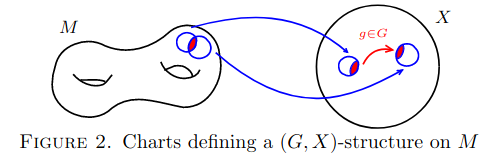
\includegraphics[scale=0.5]{GX-Charts.png}
	\end{figure}
	Other important examples include \textit{hyperbolic structures}, with $G = \PO(n,1)$ acting on $\bbH^n$, and \textit{translation structures}, with $G$ the group of translations acting on $\R^n$.
\end{example}

\subsection{Motivation}
One of the driving questions in many fields of mathematics is that of classification. In the case of geometric topology, there are two that we might focus on:
\begin{enumerate}
	\item Classify all of the model geometries $(G,X)$ that a fixed manifold $M$ may locally carry.
	\item Classify all possible $(G,X)$-structures on $M$ for a fixed model geometry $(G,X)$
\end{enumerate}
Problem (1) asks about how topology influences what geometry can exist on a space. This has led to many deep results, such as
\begin{itemize}
	\item The classical \textit{uniformization theorem}: a closed Riemann surface can carry a Euclidean, spherical, or hyperbolic structure, depending on its genus. Those which are simply connected are conformally equivalent to one of the open unit disk, the complex plane, or the Riemann sphere.
	\item Thurston's more general \textit{geometrization conjecture} (now Perelman's theorem): any closed orientable 3-manifold may be decomposed into pieces, each admitting one of eight model geometries. 
\end{itemize}

Problem (2) asks us to describe the \textit{deformation space} of $(G,X)$-structures on a manifold $M$. Even for the examples above, these spaces are quite interesting. For the case of hyperbolic structures on closed Riemann surfaces with genus $g \geq 2$, this problem is studied by Techm\"uller theory.

\subsection{Holonomy and Representation Theory}
Let $M$ be a $(G,X)$-manifold and fix a basepoint $x_0 \in M$ and a chart $\phi: U \to X$ with $x_0 \in U$. Any loop $\gamma: S^1 \to M$ starting at $x_0$ can be lifted to a path on $X$ starting at $\phi(x_0)$ by analytic continuation (walking along charts following transition maps). The last chart in this process coincides on some open set (the intersection) with $g \cdot \phi$ for some unique $g \in G$. We define a map $\hol: \pi_1(M) \to G$ called the \textit{holonomy representation} by sending $\gamma$ to $g$. It is not hard to see that this is well-define, and moreover it is unique up to conjugation by $G$. Indeed, this corresponds with our motivating examples: if $M \iso \Gamma \backslash V$ for some open $V \subset X$ and $\Gamma$ a discrete subgroup of $G$, if $V$ is simply connected, then $\hol: \pi_1(M) \to \Gamma$ is the natural identification of $\pi_1(M)$ with $\Gamma$.

We define the \textit{deformation space} $\mathscr{D}_{(G,X)}(M)$ to be the quotient of \textit{marked} $(G,X)$-structures on $M$ by the group of diffeomorphisms $\Diff_0M$ of $M$ isotopic to the identity. Holonomy defines a map $\mathscr{D}_{(G,X)}(M) \to \Hom(\pi_1(M),G)/G$ to representations of $\pi_1(M)$ into $G$ modulo conjugation by $G$. The so-called \textit{Ehresmann-Thurston} principle tells us that this map is in fact continuous (for the natural topologies on both sides), open, with discrete fibers. In particular, the set of holonomy representations of $(G,X)$-structures on $M$ is stable under small deformations.

\begin{example}
	Let $(G,X) = (PO(2,1), \bbH^2)$ and $S$ be a closed orientable connected surface of genus $g \geq 2$. All $(G,X)$-structures are complete, and their holonomy representations are Fuchsian (faithful and discrete). The deformation space $\mathscr{D}_{(G,X)}(S)$ is called the Teichm\"uller space $\mathscr{T}(S)$, and holonomy gives a homeomorphism between $\mathscr{T}(S) \iso \R^{6g - 6}$ and the space of Fuchsian representations from $\pi_1(S)$ to $G$ mod conjugation by $G$.
\end{example}


\end{document}
